\documentclass{beamer}
\usepackage[utf8]{inputenc}

\title{Strategies for computing the scalar self-force on a Schwarzschild background}
\author{Steven Dorsher}
\institute{Louisiana State University}
\date{September 26, 2017}

\begin{document}
\frame{\titlepage}


\begin{frame}
  \frametitle{Overview}
  \begin{itemize}
  \item Gravitational waves and Extreme Mass Ratio Inspirals
  \item The wave equation in flat spacetime
  \item Scalar waves on a Schwarzschild background without a source
  \item A scalar source on a Schwarzshild background on a circular orbit
  \item A scalar source on a Schwarzschild background on an eccentric orbit
  \item First order Richardson extrapolation
  \item The Discontinuous Galerkin method
  \item Fit to extend the mode sum to $\ell=\infty$
  \item Future work: a comparison of the self-consistent evolution and the geodesic evolution
  \end{itemize}
\end{frame}


\begin{frame}
  \frametitle{Extreme Mass Ratio Inspirals}
  \begin{figure}
    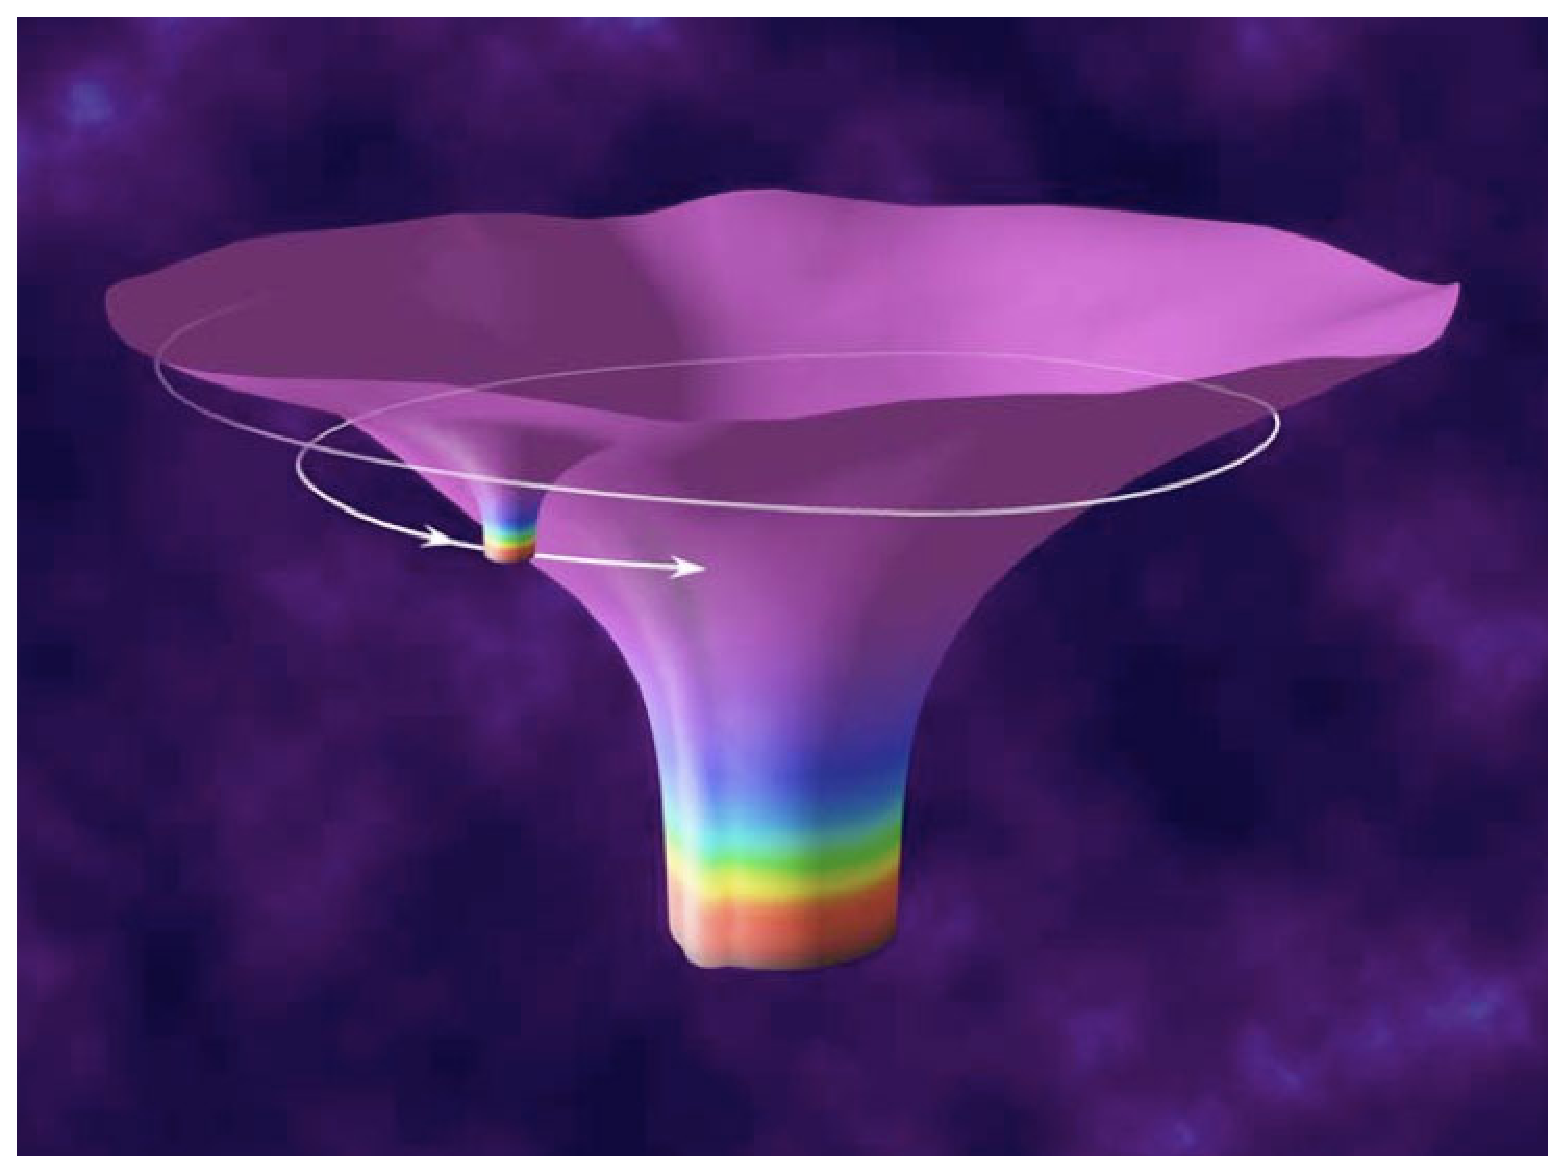
\includegraphics[width=4.0in]{EMRI}
    \citation{Extreme Mass Ratio Inspiral, $\mu=m/M\sim 10^{-4}$ to $10^{-6}$, Artist's rendition, Wikipedia}
  \end{figure}
\end{frame}

\begin{frame}
  \frametitle{Laser Interferometer Space Antenna}
  \begin{figure}
    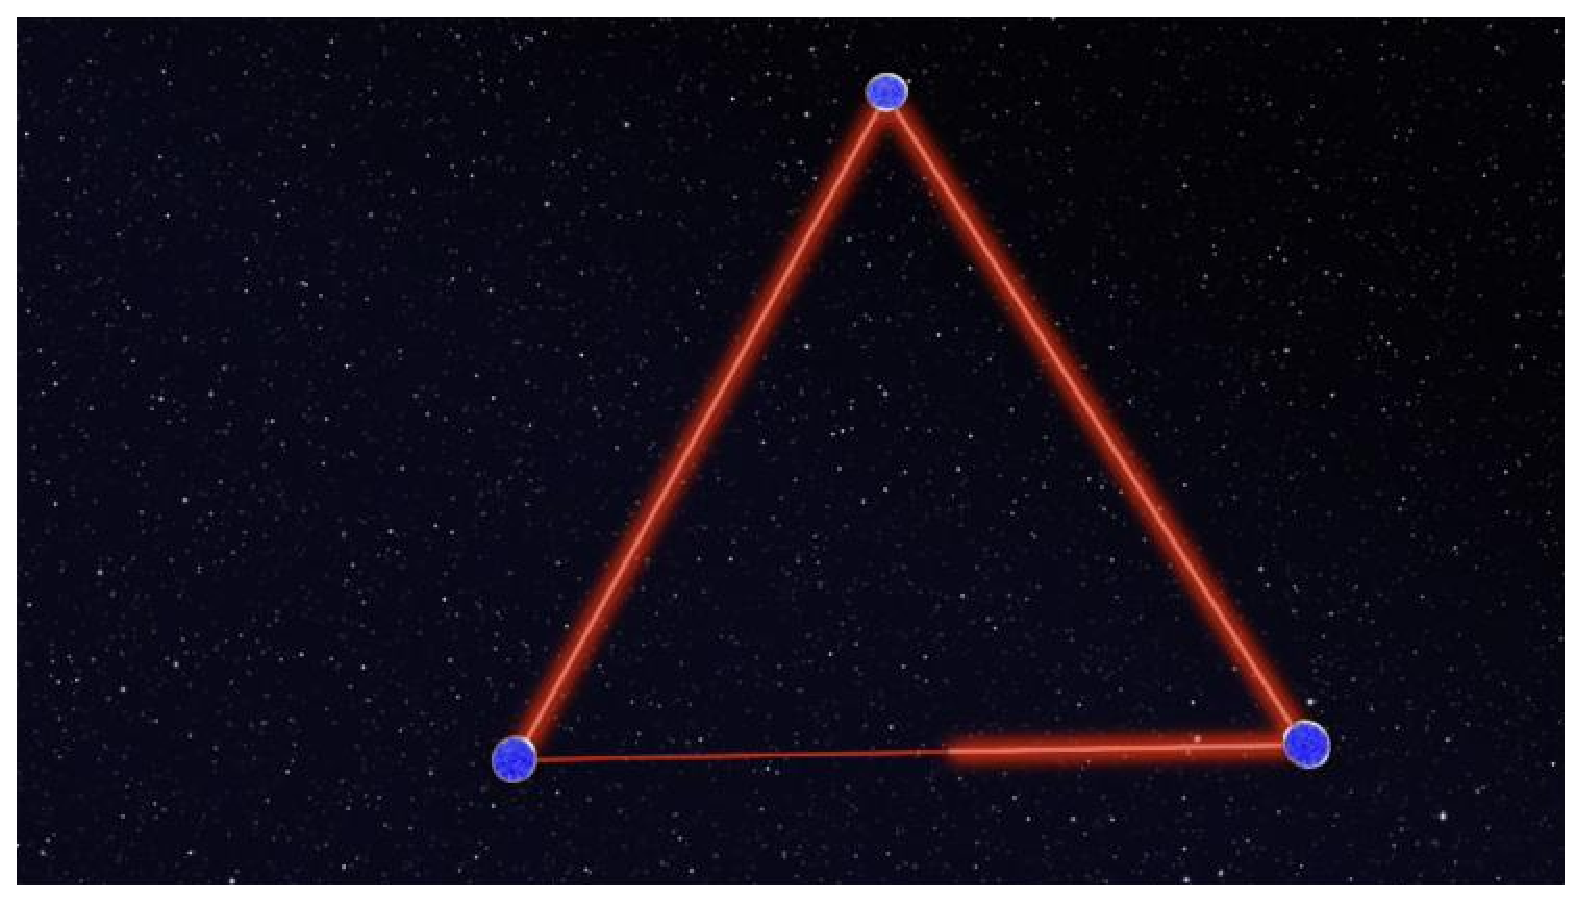
\includegraphics[width=4.0in]{eLISA}
    \caption{Laser Interferometer Space Antenna, which will operate around launches in early 2030's, ESA-NASA partnership, will detect EMRI's}
  \end{figure}
\end{frame}


\begin{frame}
  \frametitle{Gravitational Waves}
  \begin{figure}
    \includegraphics[width=4.0in]{LIGOGRtest.png}
    \caption{LIGO detection, September 14, 2015. General relativity was tested by comparing inpsiral with merger/ringdown phases.}
  \end{figure}
\end{frame}

\begin{frame}
  \frametitle{Self-force}
  \begin{itemize}
  \item The self-force is a particle's interaction with its own field
  \item applies to scalar, electromagnetic, and tensor fields on a gravitational background
  \item motion $\rightarrow$ radiation $\rightarrow$ energy and angular momentum loss $\rightarrow$ inspiral
  \item electromagnetic or gravitational field: source from perturbation theory
  \item scalar: delta function source
  \end{itemize}
\end{frame}

\begin{frame}
  \frametitle{Approximations and Goals}
  The long term goal for the field is to generate extremely precise EMRI gravitational wave templates for LISA.

  Approximations:
  \begin{itemize}
  \item scalar rather than tensor waves ($\Psi$ rather than $h_{\mu\nu}$)
  \item non-rotating black holes: Schwarzschild spacetime
  \item self-force causes a particle to inspiral as it emits radiation
  \item we use the Detweiler-Whiting effective source as implemented by Barry Wardell
  \item Niels Warburton assumes: the particle has been on the same geodesic for all time when he calculates the self-force
  \end{itemize}
  
  Our goal is to implement a highly accurate self-consistent scalar evolution of an EMRI using the self-force method and do a comparison study of the self-force at the location of the particle with Niels Warburton.

  First: some simpler wave equation and self-force problems, in flat and curved spacetime
  
\end{frame}

\begin{frame}
  \frametitle{Wave equation in flat spacetime}
  For no source, the D'Alembertial equals zero:
  \begin{equation}
    \Box\Psi=0
  \end{equation}
  In 1-dimension:
  \begin{equation}
    \frac{\partial^2\Psi}{\partial t^2}-\frac{\partial^2\Psi}{\partial x^2}=0
  \end{equation}
  Rewrite as ODE
  \begin{eqnarray}
    \partial_t \psi &= \rho\nonumber\\
    \partial_t \rho &= \partial_r \phi\nonumber\\
    \partial_t \phi &= \partial_r \rho
  \end{eqnarray}
  Refer to $u=(\psi,\rho,\phi)$ as the state vector.
\end{frame}

\begin{frame}
  \frametitle{Flat space evolution}
  \begin{figure}
    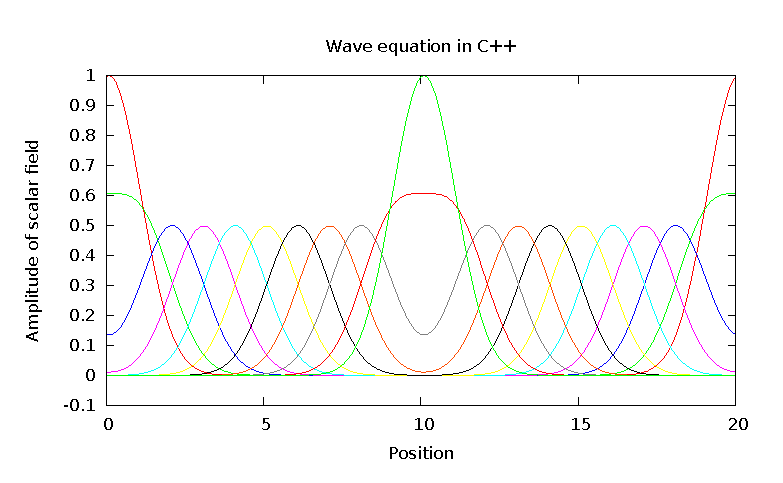
\includegraphics[width=4.0in]{gaussWave}
    \caption{Gaussian initial conditions, flat spacetime}
  \end{figure}
\end{frame}



\begin{frame}
  \frametitle{The Discontinuous Galerkin (DG) method}
  \begin{itemize}
  \item Method for solving ODEs dependent on space and time.
  \item Break space into evenly spaced elements.
  \item Each element of order $N$ has $N+1$ unevenly spaced nodes.
  \item $N+1$ interpolating polynomials run through these nodes to represent the values of the state vector.
  \item Numerical fluxes handle the flow of information through the ends of elements and naturally account for discontinuities that are allowed to occur there.
  \item The DG method returns a derivative matrix that takes a derivative across an element and a lift matrix that accounts for numerical fluxes,
  \item Beneficial because it has truncation error that decreases exponentially with DG order $N$ and because it naturally handles discontinuities in $\phi$ and $\rho$. 
  \end{itemize}
\end{frame}

\begin{frame}
  \frametitle{Flat spacetime error convergence}
  \begin{figure}
    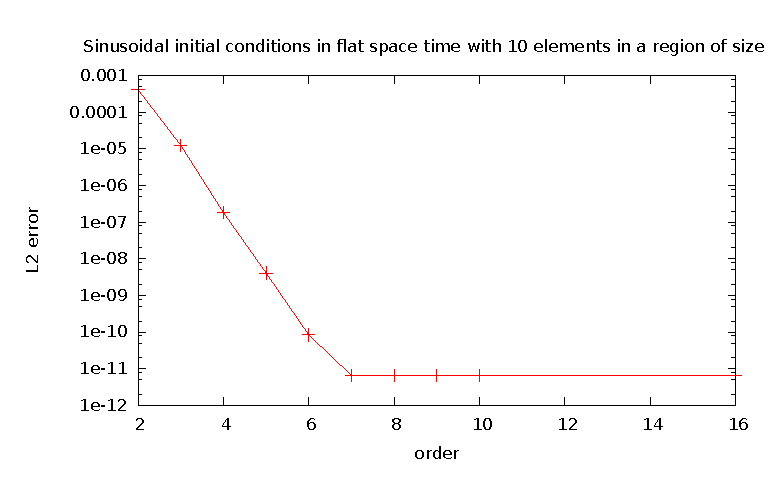
\includegraphics[width=4.0in]{sinL2WTorder}
    \caption{$L_2$ error converges exponentially until it hits roundoff noise with DG order for sinusiodal initial conditions with ten elements of size $h=0.01$.}
  \end{figure}
\end{frame}



\end{document}
